%   ------------------------------------------------------------------------
\FloatBarrier
\subsection{Geração da animação das portas abrindo}
\label{s.gemini.animacaoPorta}

Foi tentado criar animações dos sprites de diferentes portas (Figuras \ref{fig:geminiProPortaA} a \ref{fig:geminiProTutorial}) abrindo, em pontos de vista distintos. Durante os testes iniciais, os experimentos focaram na produção da animação da porta A em front view (Figura \ref{fig:geminiProPortaA}).

O prompt usado inicialmente foi simples e direto, apenas apontando o que é o sprite e requisitando a animação específica. Baseado nos erros do resultado gerado, foram adicionados detalhes mais específicos na instrução com o intuito de corrigir os erros, como pode ser visto na Figura \ref{fig:geminiProPortaAMudaPrompt}. A consistência do sprite se manteve alta durante todo o experimento, apesar de não apresentar uma animação coerente com o estilo pixel art e os resultados iniciais apresentarem imprecisões no movimento por causa da interpretação incorreta sobre a posição da maçaneta e o lado para o qual a porta deveria abrir.

\begin{figure}[htbp]
    \centering
    \caption{\small Demonstração da edição do prompt baseado no resultado do vídeo gerado no GeminiPro}
    \label{fig:geminiProPortaAMudaPrompt}
    \begin{subfigure}{0.3\linewidth}
        \centering
        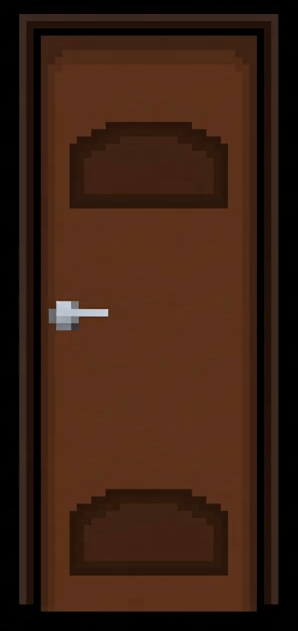
\includegraphics[width=1\linewidth]{figs/geminiPro/chat7/macanetaLadoErrado.PNG}
        \caption{\small Porta com a maçaneta do lado oposto em relação ao sprite original}
        \label{fig:geminiProPortaAMudaPromptErro}
    \end{subfigure}\hfill
    \begin{subfigure}{0.65\linewidth}
        \centering
        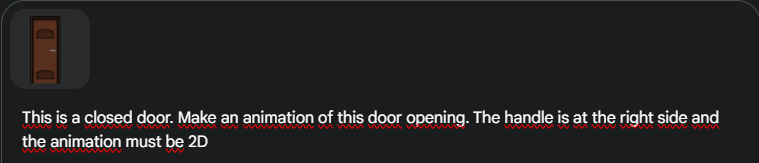
\includegraphics[width=1\linewidth]{figs/geminiPro/chat7/tela20.PNG}
        \caption{\small Prompt especificando lado certo da maçaneta}
        \label{fig:geminiProPortaAMudaPromptNovo}
    \end{subfigure}\hfill

    \legend{\small Fonte: Elaborada pela autora.}
\end{figure}

Essa estratégia mostrou-se extremamente efetiva, sendo possível gerar uma animação satisfatória em apenas três interações. Todos os testes e resultados\footnote{\url{https://drive.google.com/drive/folders/10Whp-LvVw9JMa_Pc7ZjOHjllu-G5htA6?usp=drive_link}} podem ser consultados nas Figuras \ref{fig:geminiProPortaA1} a \ref{fig:geminiProPortaA3} no Apêndice \ref{ap.telasIA}.

O sprite sheet do melhor resultado foi obtido pela ferramenta ezgif, como pode ser visto na Figura \ref{fig:geminiProPortaASpriteSheet}. O fundo foi removido utilizando a ferramenta Photoroom\footnote{\url{https://app.photoroom.com/create}} (Figura \ref{fig:geminiProPortaASpriteSheetSemFundo}) e o resultado foi transformado em pixel perfect pela ferramenta Pixilart (Figura \ref{fig:geminiProPortaASpriteSheetPixel}). 

\begin{figure}[htbp]
    \centering
    \caption{\small Sprite sheet da animação da porta A abrindo gerada no Gemini Pro}
    \label{fig:geminiProPortaASpriteSheet}
    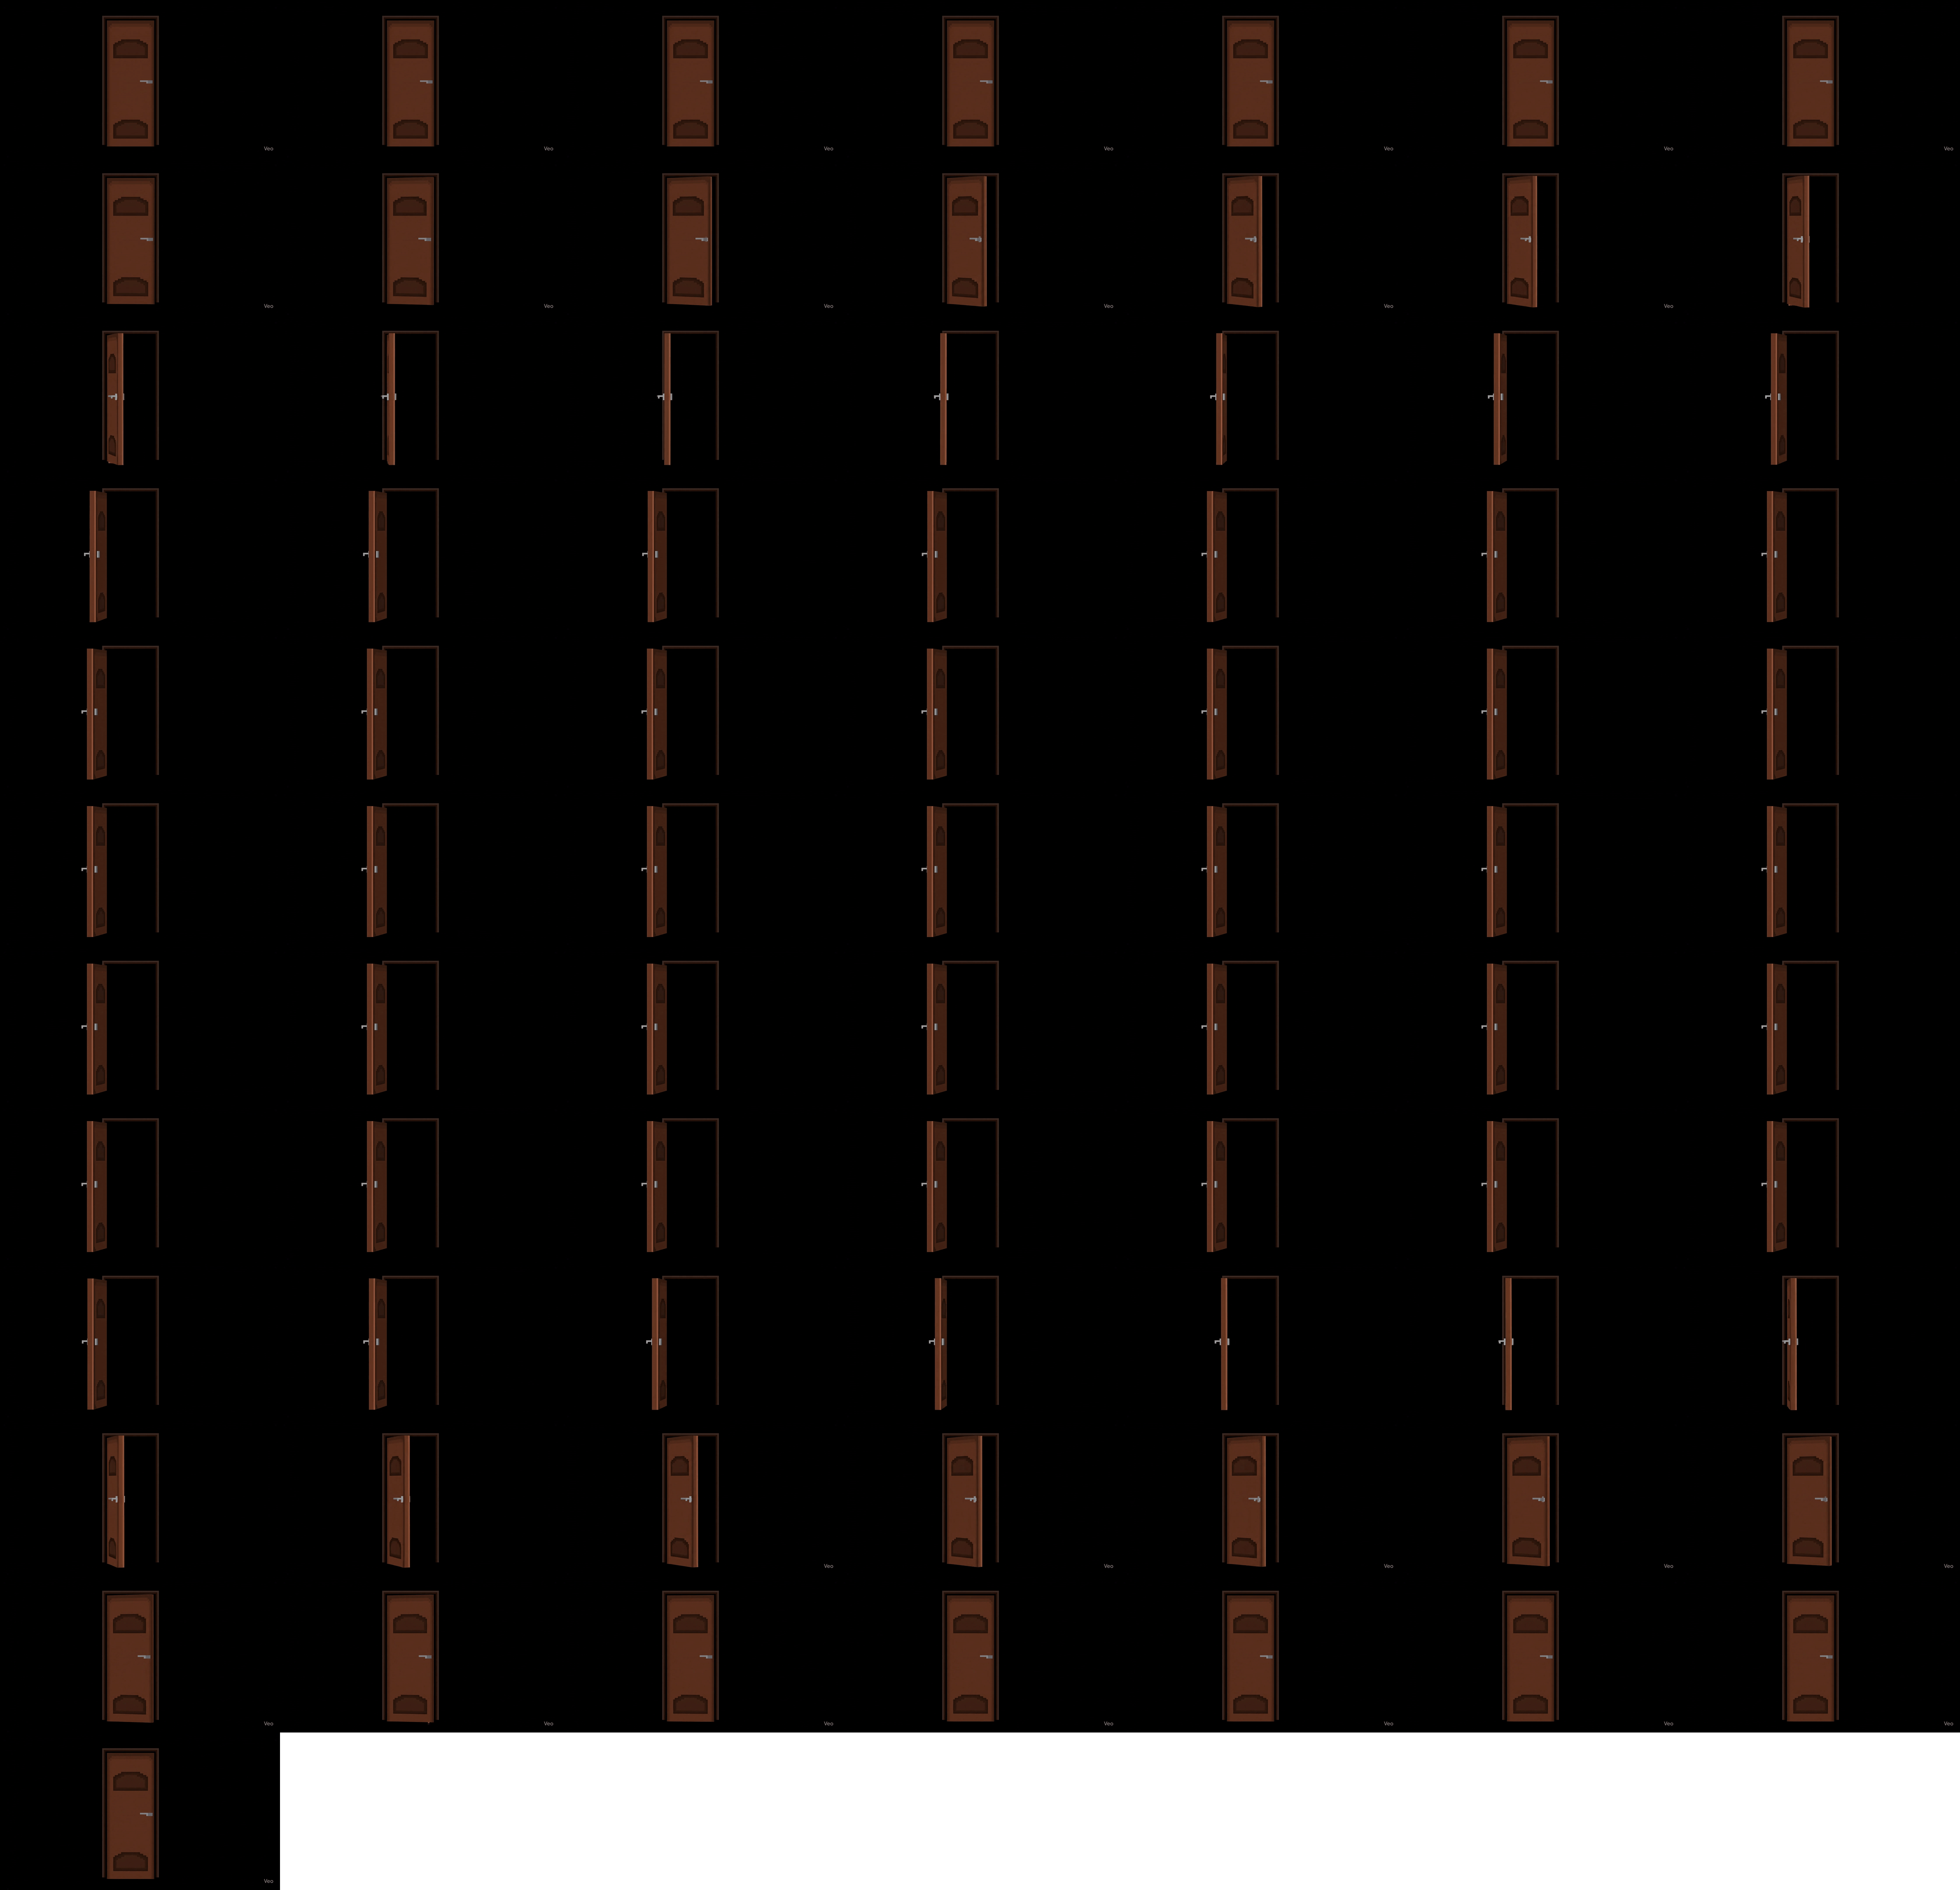
\includegraphics[width=0.5\linewidth]{figs/geminiPro/sprite sheet/door_sprite_sheet.png}
    \legend{\small Fonte: Elaborada pela autora, utilizando a ferramenta ezgif.}
\end{figure}

\begin{figure}[htbp]
    \centering
    \caption{\small Sprite sheet sem fundo da animação da porta A abrindo}
    \label{fig:geminiProPortaASpriteSheetSemFundo}
    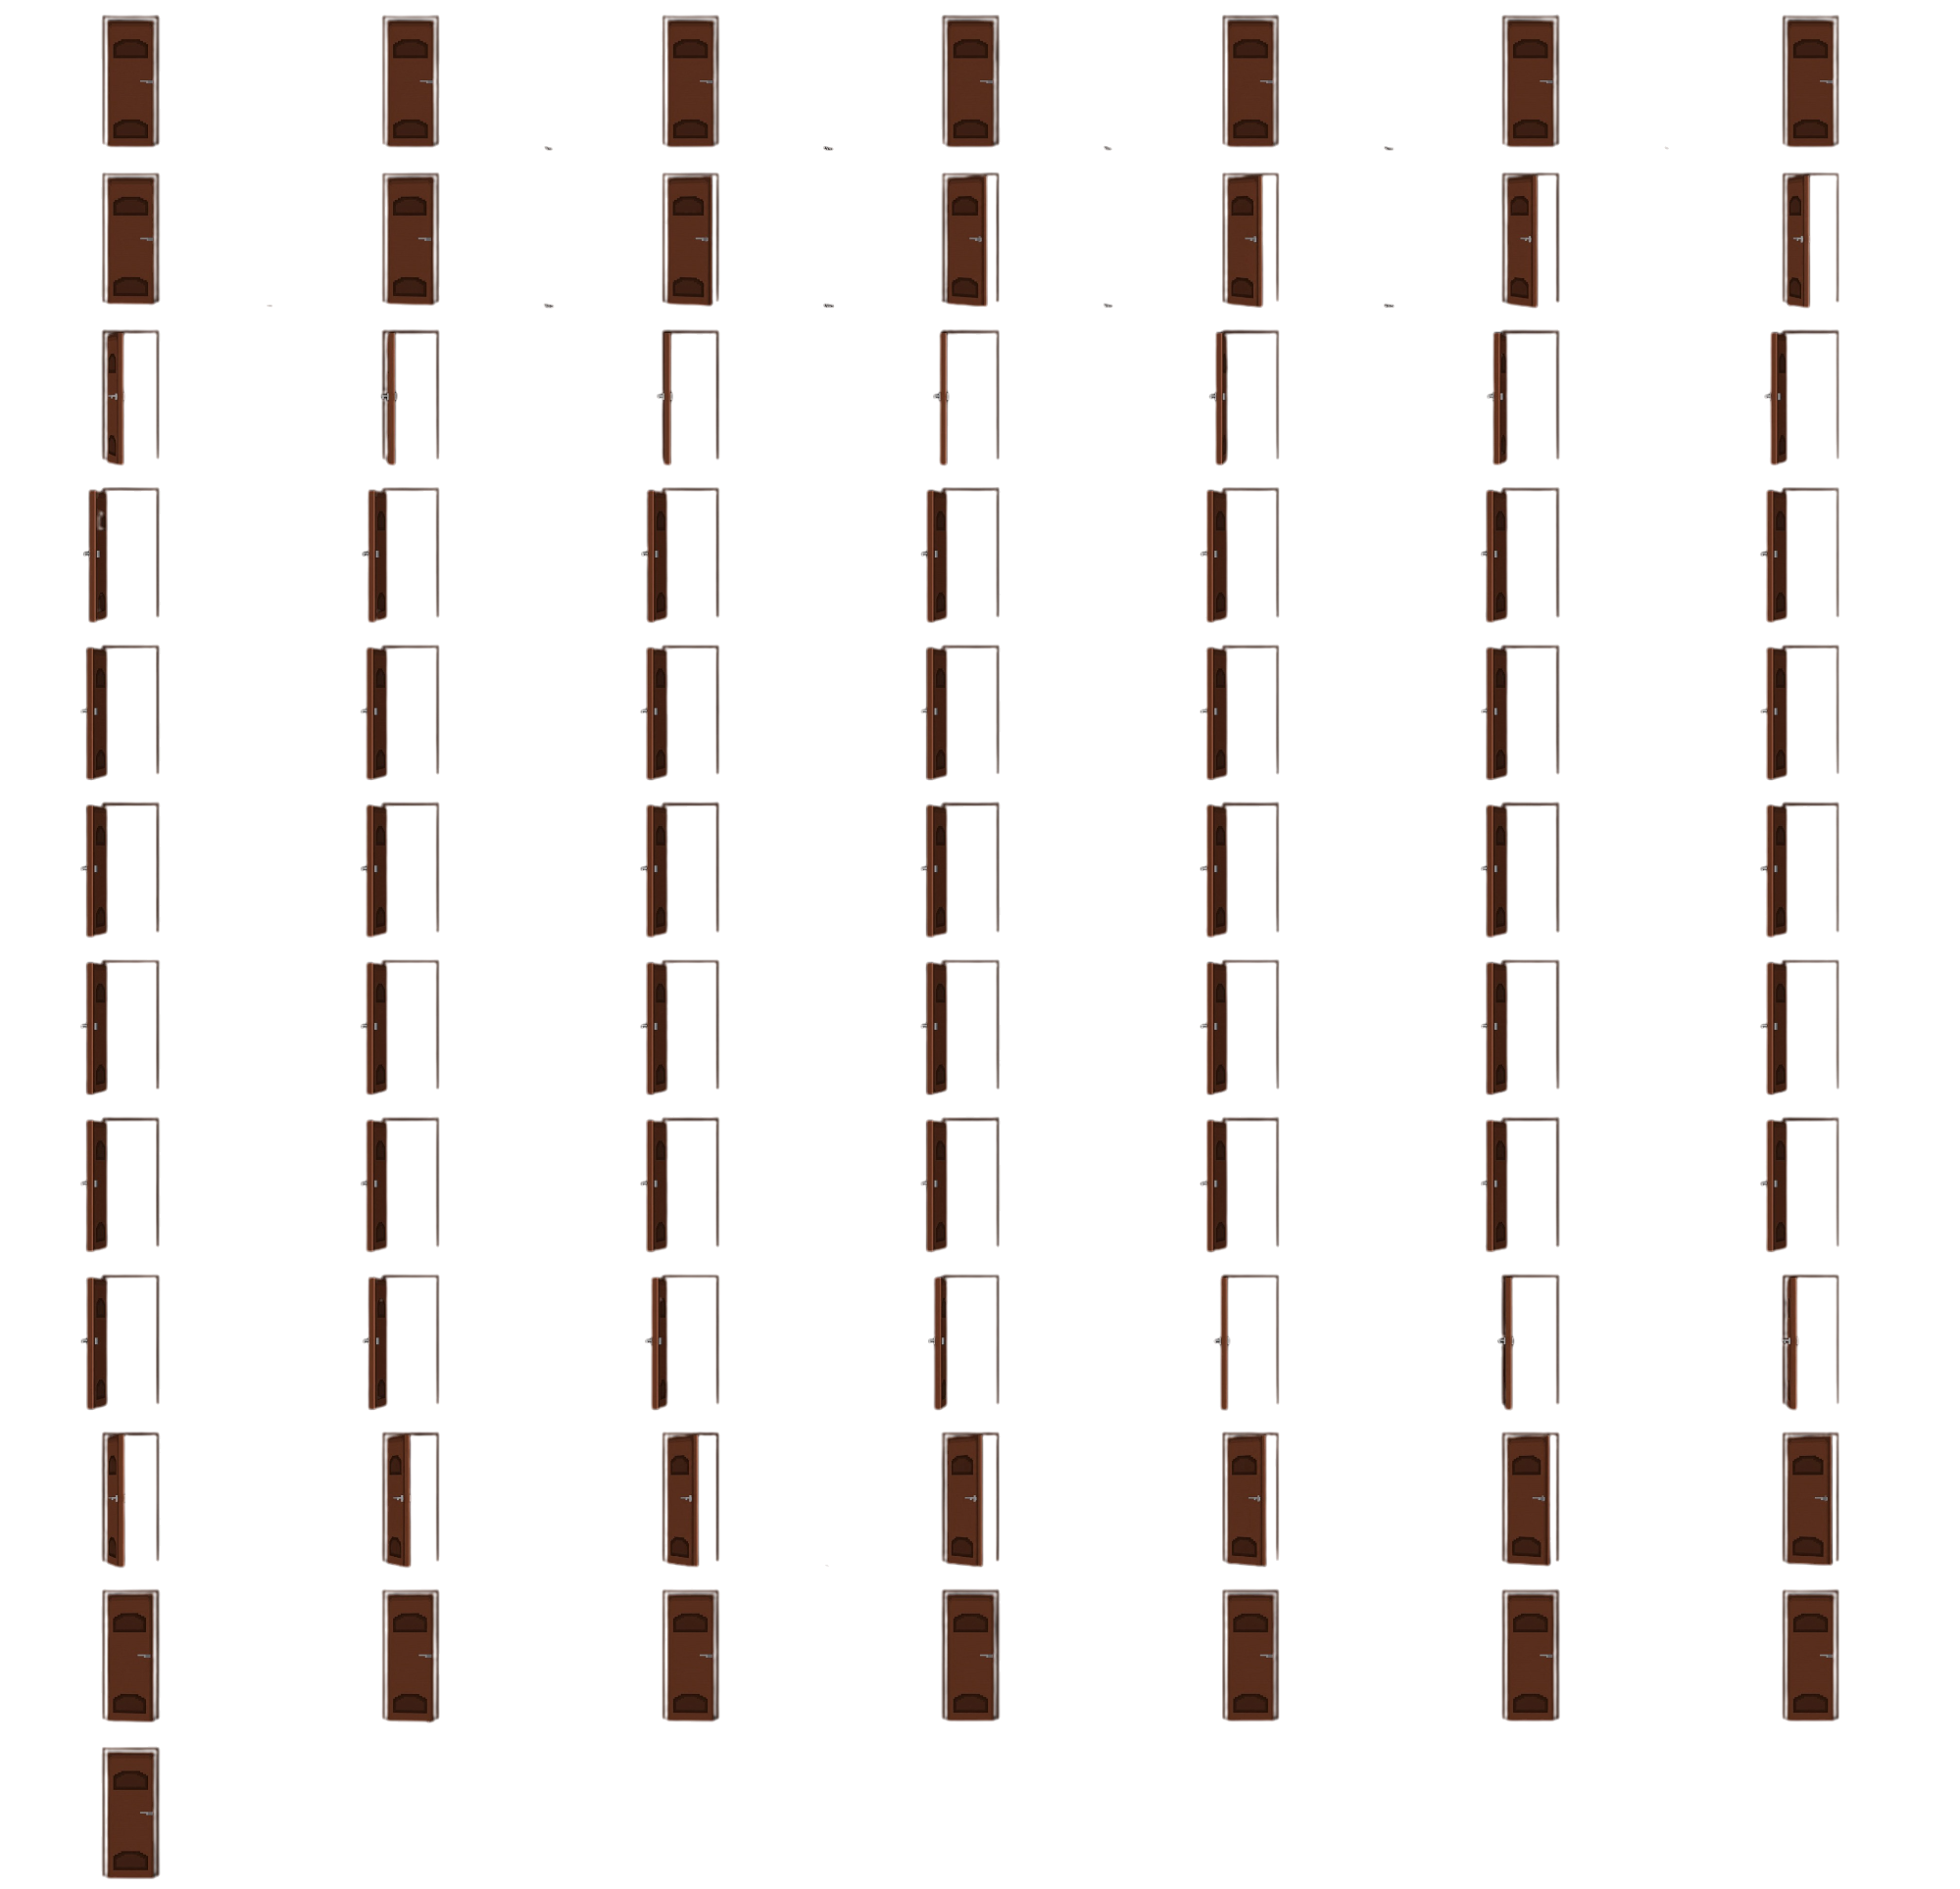
\includegraphics[width=0.5\linewidth]{figs/geminiPro/sprite sheet/door_spriteSheet_semFundo-Photoroom.png}
    \legend{\small Fonte: Elaborada pela autora, utilizando a ferramenta Photoroom.}
\end{figure}

\begin{figure}[htbp]
    \centering
    \caption{\small Sprite sheet pixelizado da animação da porta A abrindo}
    \label{fig:geminiProPortaASpriteSheetPixel}
    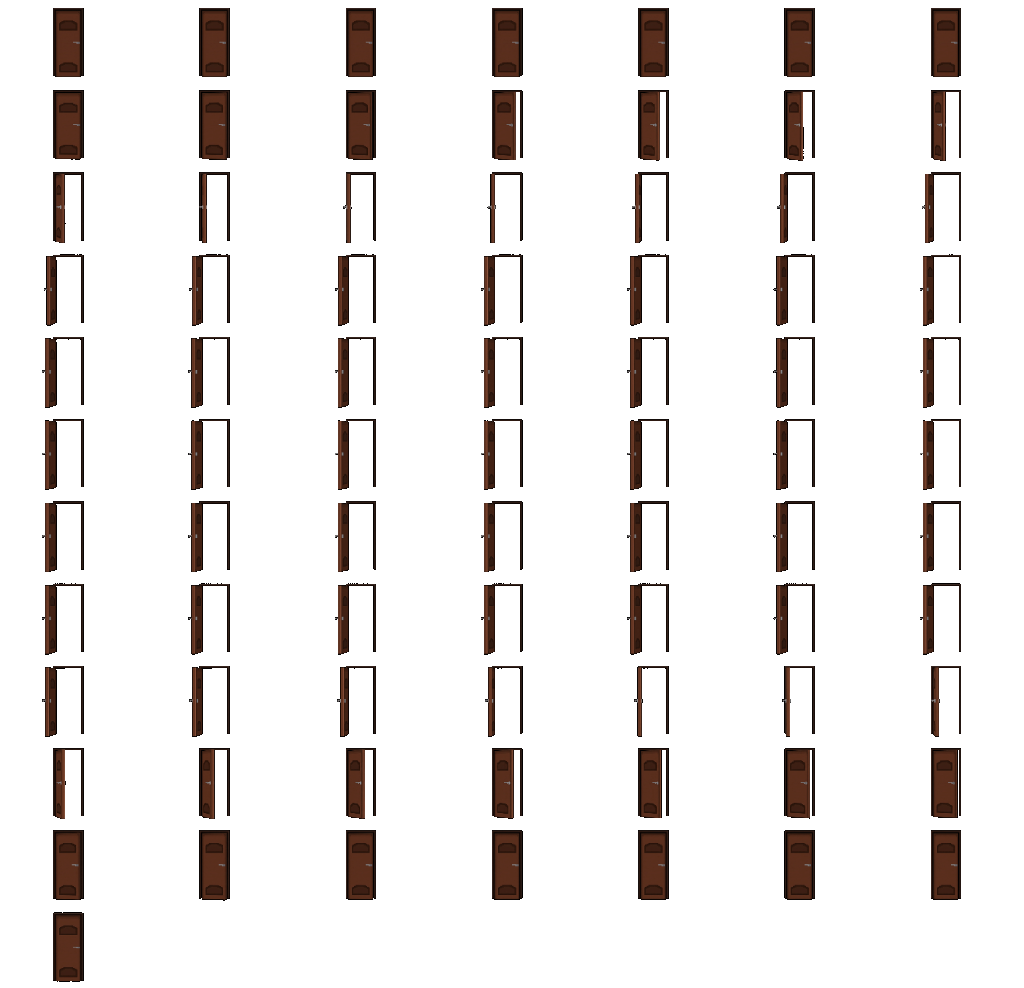
\includegraphics[width=0.8\linewidth]{figs/geminiPro/sprite sheet/door_fundo_transparente_pixel.png}
    \legend{\small Fonte: Elaborada pela autora, utilizando a ferramenta Pixilart.}
\end{figure}



Nesse mesmo editor, foi aperfeiçoada a animação para manter a porta com tamanho correspondente ao do sprite original durante todo o movimento de abertura. Isso foi feito colocando o sprite da porta fechada lado a lado com o primeiro quadro da animação e adicionando modificações conforme às mudanças dos frames. Na Figura \ref{fig:geminiProPortaASpriteSheetAjuste} pode ser visto lado a lado o quadro do vídeo gerado (sprite menor, à esquerda) com o quadro editado (sprite maior, à direita). A Figura \ref{fig:geminiProPortaASpriteSheetFinal} apresenta o sprite sheet final da animação.

\begin{figure}[htbp]
    \centering
    \caption{\small Comparação dos quadros da animação gerada antes da edição (sprite menor) e depois da edição (sprite maior)}
    \label{fig:geminiProPortaASpriteSheetAjuste}
    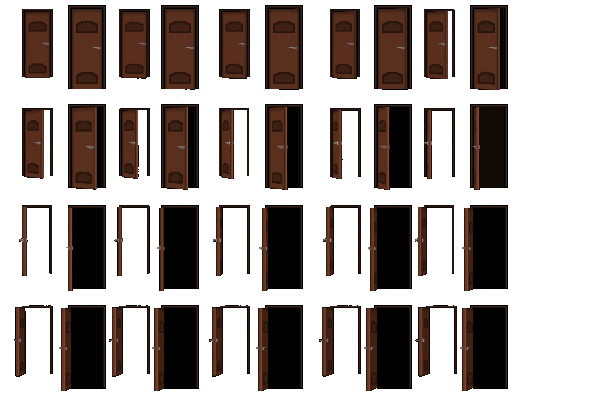
\includegraphics[width=0.8\linewidth]{figs/geminiPro/sprite sheet/door_ajuste.png}
    \legend{\small Fonte: Elaborada pela autora, utilizando a ferramenta Pixilart.}
\end{figure}

\begin{figure}[htbp]
    \centering
    \caption{\small Sprite sheet finalizado da animação da porta A abrindo}
    \label{fig:geminiProPortaASpriteSheetFinal}
    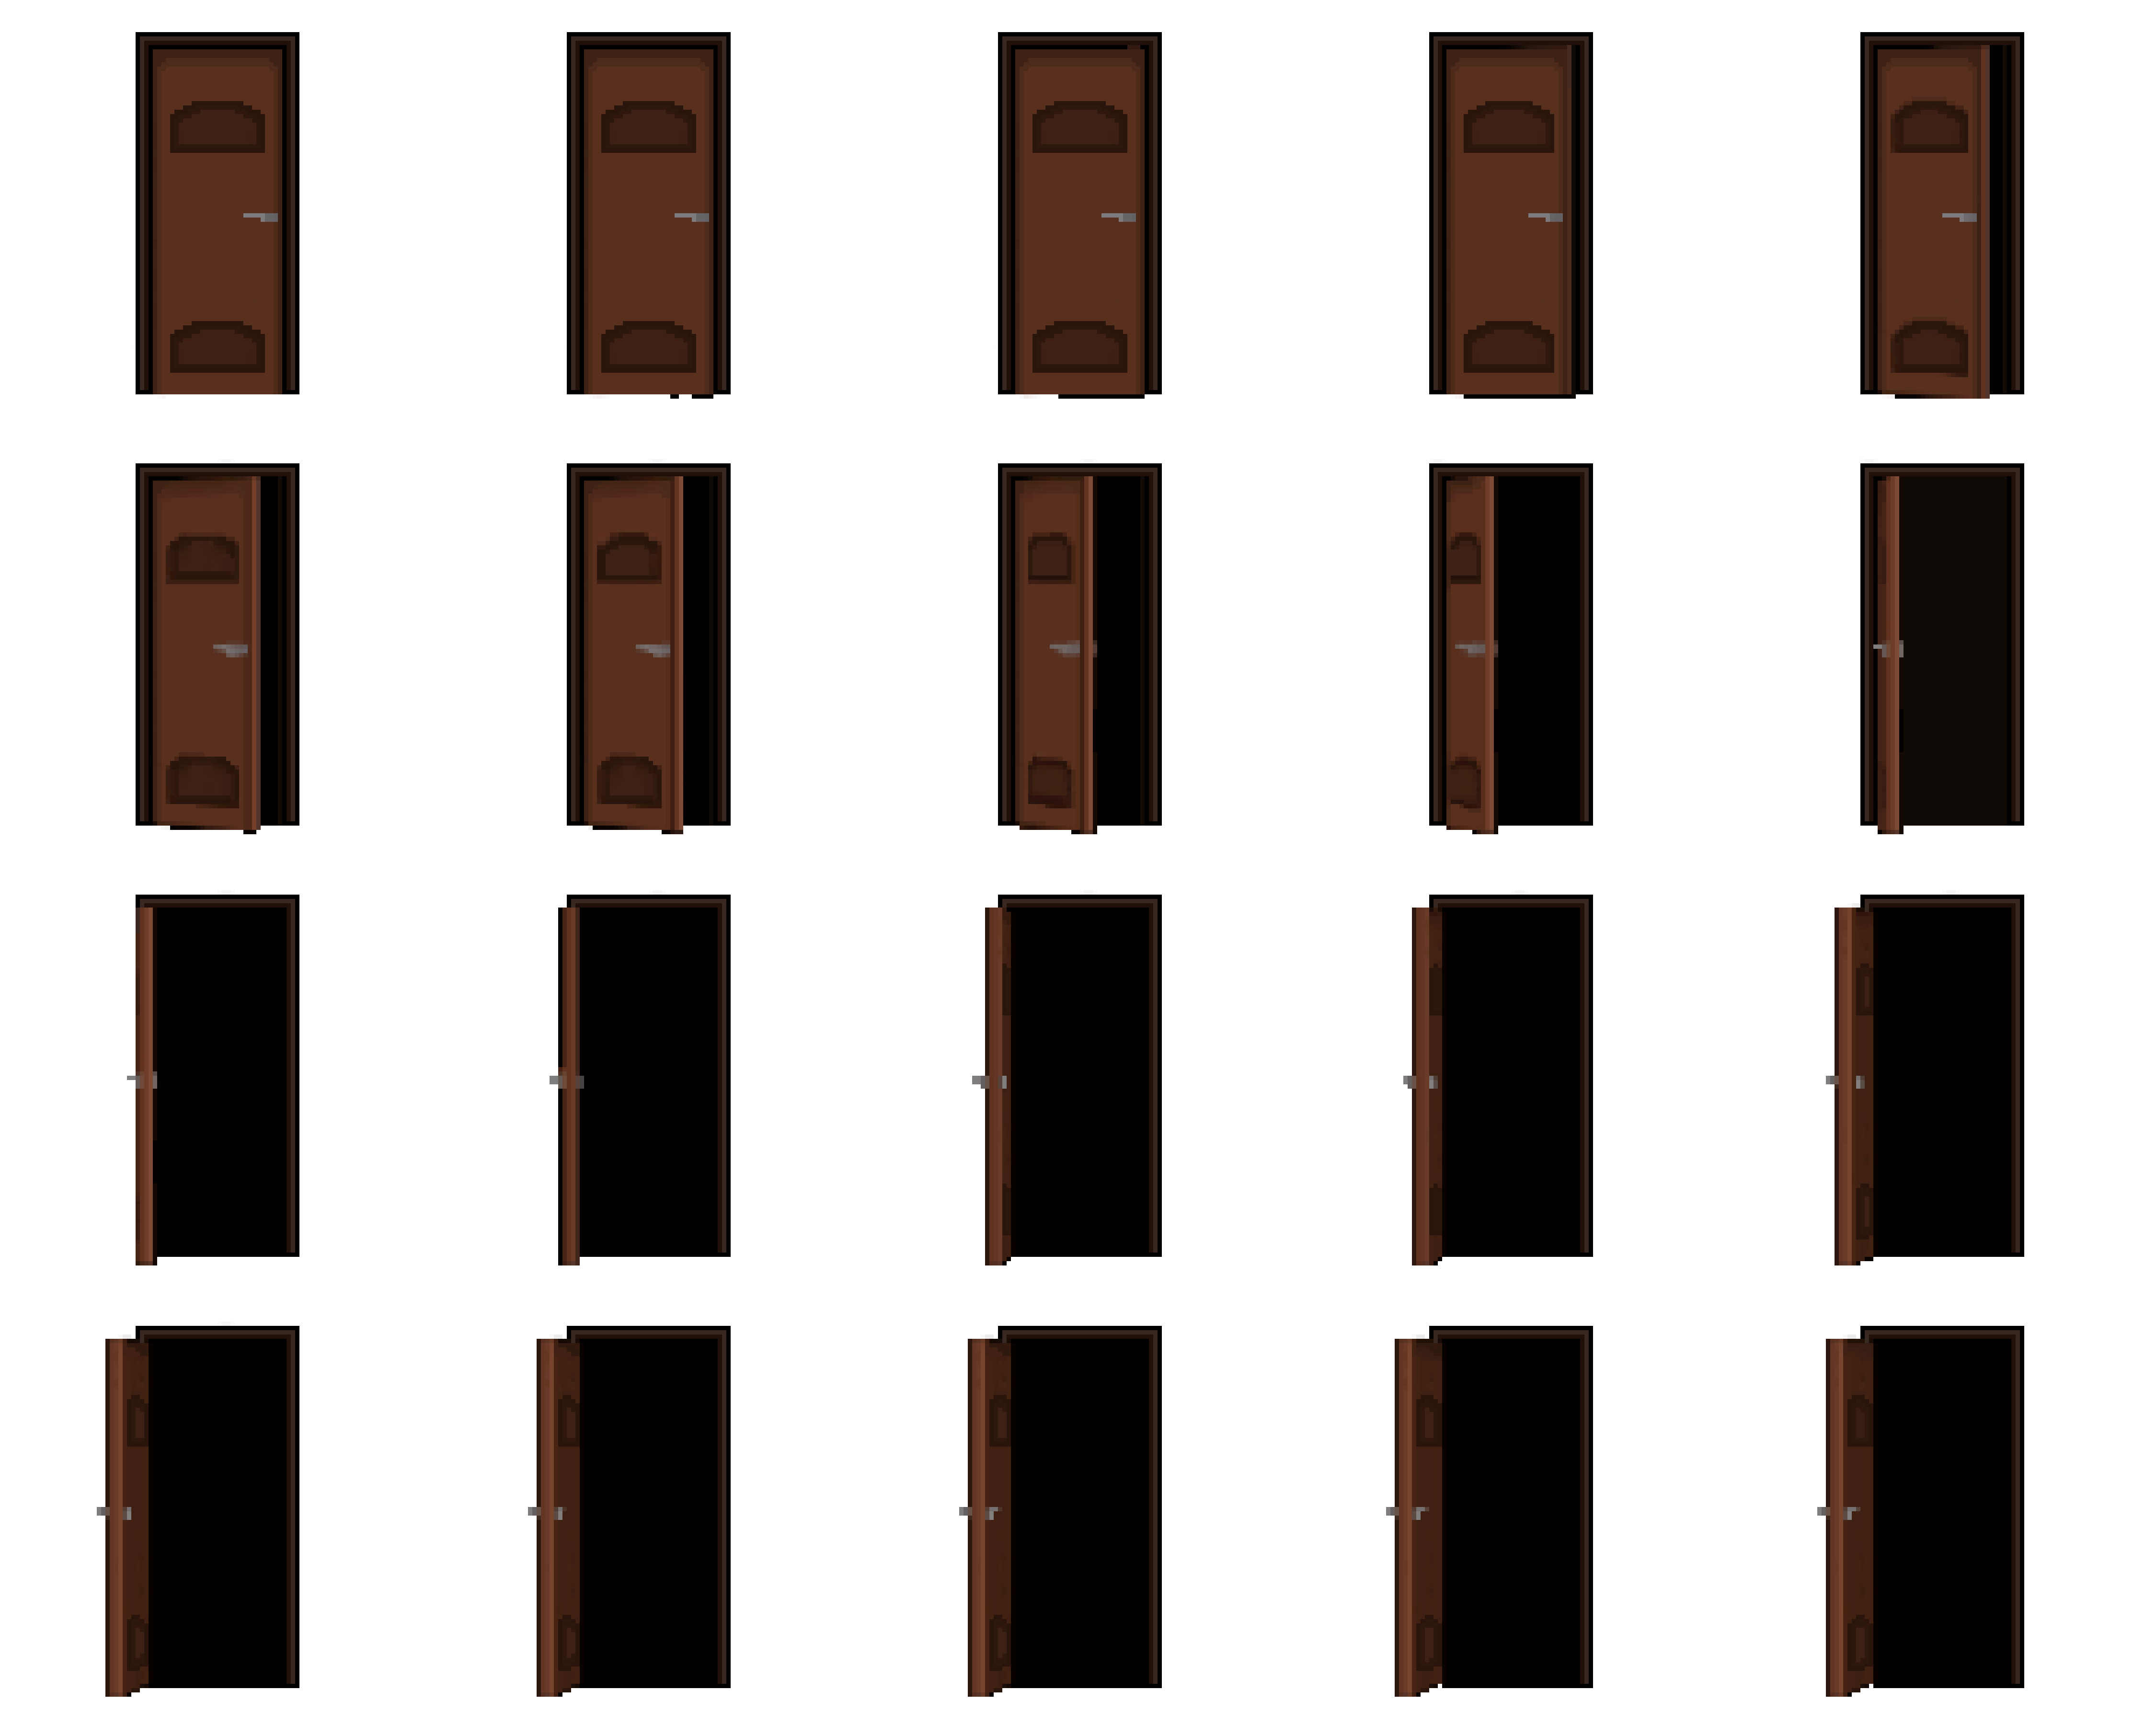
\includegraphics[width=0.8\linewidth]{figs/geminiPro/sprite sheet/door_pixel_correcao.png}
    \legend{\small Fonte: Elaborada pela autora, utilizando a ferramenta Pixilart.}
\end{figure}

Esse processo mostra como a IA é apenas uma ferramenta para auxiliar o desenhista na produção da animação, criando uma base para ser editada e aprimorada pelo artista, fazendo com que ele não tenha que desenhar cada frame do zero e oferecendo uma referência visual personalizada de como cada quadro da animação deve ficar, de forma a ainda serem permitidas customizações e detalhes específicos visionados pelo desenhista.

A bateria de testes posterior focou na geração da animação da Porta B abrindo em side view (Figura \ref{fig:geminiProPortaB}). Durante o jogo, a porta vai abrir para o lado oposto ao personagem e para a esquerda do mesmo, de forma que o sprite da porta ficaria na frente do sprite do personagem quando ele passar por ela. Uma das grandes dificuldades durante essa etapa foi conseguir explicar de maneira clara como a porta deveria abrir. 

Apesar da porta abrir para a esquerda do personagem, no prompt foi instruído para a porta abrir para a direita. O motivo disso foi que o lado esquerdo do personagem equivale ao lado direito da imagem em side view, como detalhado na Figura \ref{fig:geminiProPortaBEsquema}


\begin{figure}[htbp]
    \centering
    \caption{\small Esquema mostrando animação da porta abrindo em diferentes ângulos}
    \label{fig:geminiProPortaBEsquema}
    \begin{subfigure}{1\linewidth}
        \centering
        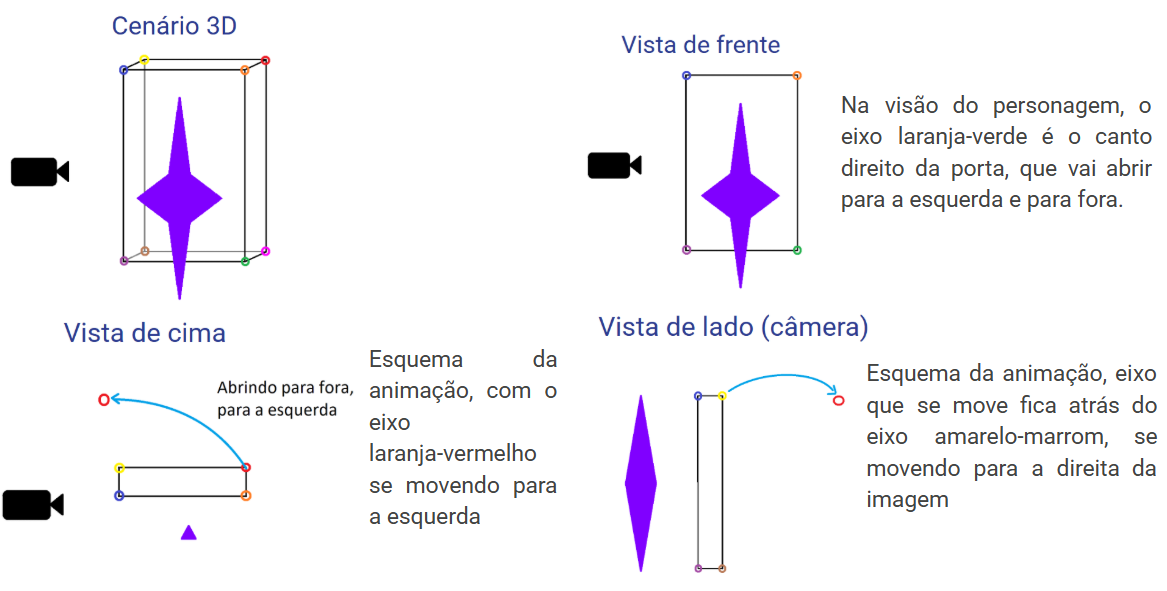
\includegraphics[width=1\linewidth]{figs/geminiPro/chat7/esquemaPortaSideViewCompleto.PNG}
        \caption{\small Esquema}
        \label{fig:geminiProPortaBEsquemaFigura}
    \end{subfigure}\hfill
    \begin{subfigure}{0.3\linewidth}
        \centering
        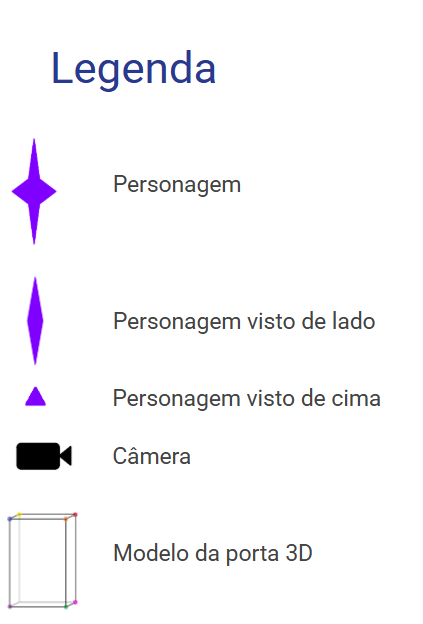
\includegraphics[width=1\linewidth]{figs/geminiPro/chat7/esquemaPortaSideViewLegenda.PNG}
        \caption{\small Legenda}
        \label{fig:geminiProPortaBEsquemaLegenda}
    \end{subfigure}\hfill

    \legend{\small Fonte: Elaborada pela autora.}
\end{figure}

O prompt inicial era focado em descrever a porta, o ambiente e o quadro final. O resultado\footnote{\url{https://drive.google.com/file/d/1bqLKpgjRTf3mpunUhvbB8464SkbnOmIh/view?usp=sharing}} apresentou erros na compreensão do sprite, formando uma porta dupla e em vista frontal ao mesmo tempo em que a abertura ocorria (Figura \ref{fig:geminiProPortaBDupla}). A instrução foi ajustada, removendo qualquer trecho que gerasse ambiguidade, e mais testes foram realizados. O novo vídeo\footnote{\url{https://drive.google.com/file/d/1TkvEqaEhS6mMNmAyHgM2NDxr674SkwTs/view?usp=sharing}} gerado corrigiu a inconsistência do sprite, porém criou um movimento impreciso, realizando a abertura em uma direção distinta da desejada. Ambos os experimentos descritos são encontrados na íntegra nas Figuras \ref{fig:geminiProPortaB1} e \ref{fig:geminiProPortaB2} no Apêndice \ref{ap.telasIA}.

\begin{figure}[htbp]
    \centering
    \caption{\small Porta dupla na animação gerada no Gemini Pro}
    \label{fig:geminiProPortaBDupla}
    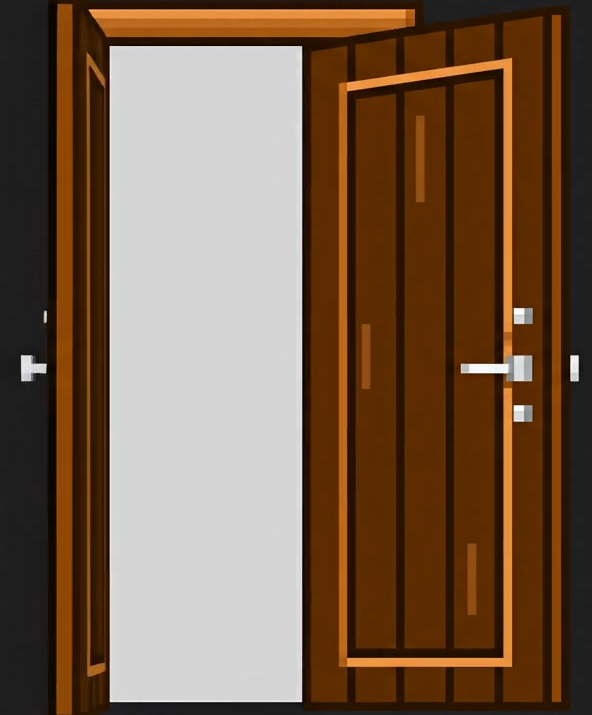
\includegraphics[width=0.4\linewidth]{figs/geminiPro/chat7/portaDupla.PNG}
    \legend{\small Fonte: Elaborada pela autora, utilizando a ferramenta Gemini Pro.}
\end{figure}

Mais edições foram feitas ao prompt, focando na descrição da animação e na especificação da direção de cada movimento. Os resultados\footnote{\url{https://drive.google.com/drive/folders/1fwdzRZ7PL-uzQBVbJo5bKBHL_hjchn1V?usp=sharing}}, porém, continuaram a apresentar as mesmas falhas na precisão do sprite e do movimento, como pode ser verificado nas Figuras \ref{fig:geminiProPortaB3} a \ref{fig:geminiProPortaB6} no Apêndice \ref{ap.telasIA}.

Após mais algumas tentativas, a instrução visou forçar a IA a manter o eixo frontal fixo, além de repetir a descrição do movimento. A maior parte dos vídeos gerados\footnote{\url{https://drive.google.com/drive/folders/1PQiVTqdHLN8fW6p62TypZ2Ia-WW8ynjs?usp=sharing}} continuou a não formar a movimentação precisa. Porém, uma das animações\footnote{\url{https://drive.google.com/file/d/1bBW7_HzSdrtaU5Tl3Lj8auSoJJEMxYSC/view?usp=sharing}} fez a abertura na direção correta após uma rápida deformação (Figura \ref{fig:geminiProPortaBDeformacao}), que poderia ser removida com uma leve edição. As Figuras \ref{fig:geminiProPortaB7} a \ref{fig:geminiProPortaB9} mostram os testes completos.

\begin{figure}[htbp]
    \centering
    \caption{\small Deformação na porta B na animação gerada no Gemini Pro}
    \label{fig:geminiProPortaBDeformacao}
    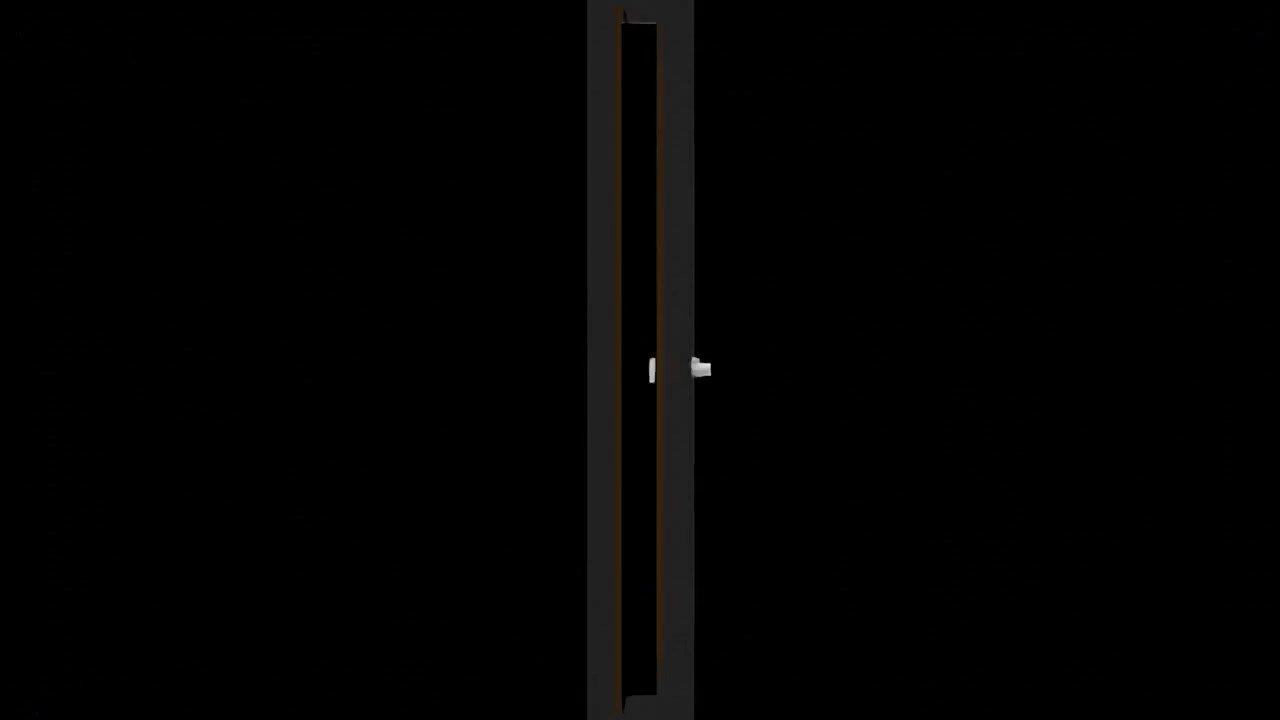
\includegraphics[width=0.6\linewidth]{figs/geminiPro/chat7/portaDeformacao.jpg}
    \legend{\small Fonte: Elaborada pela autora, utilizando a ferramenta Gemini Pro.}
\end{figure}

Para isso, foi extraído o sprite sheet do vídeo (Figura \ref{fig:geminiProPortaBSpriteSheet}), utilizando a ferramenta ezgif (mencionada anteriormente). Essa imagem foi convertida para o padrão pixel perfect através do Pixilart, onde também foi removido o fundo e cortado o trecho para manter apenas os frames sem deformação, como mostra a Figura \ref{fig:geminiProPortaBSpriteSheetPixel}. Após isso, a animação é exportada para o Pixel Lab para mais ajustes (detalhado na Seção \ref{s.pixelLab.edicao}).

\begin{figure}[htbp]
    \centering
    \caption{\small Sprite sheet da animação da Porta B abrindo gerada no Gemini Pro}
    \label{fig:geminiProPortaBSpriteSheet}
    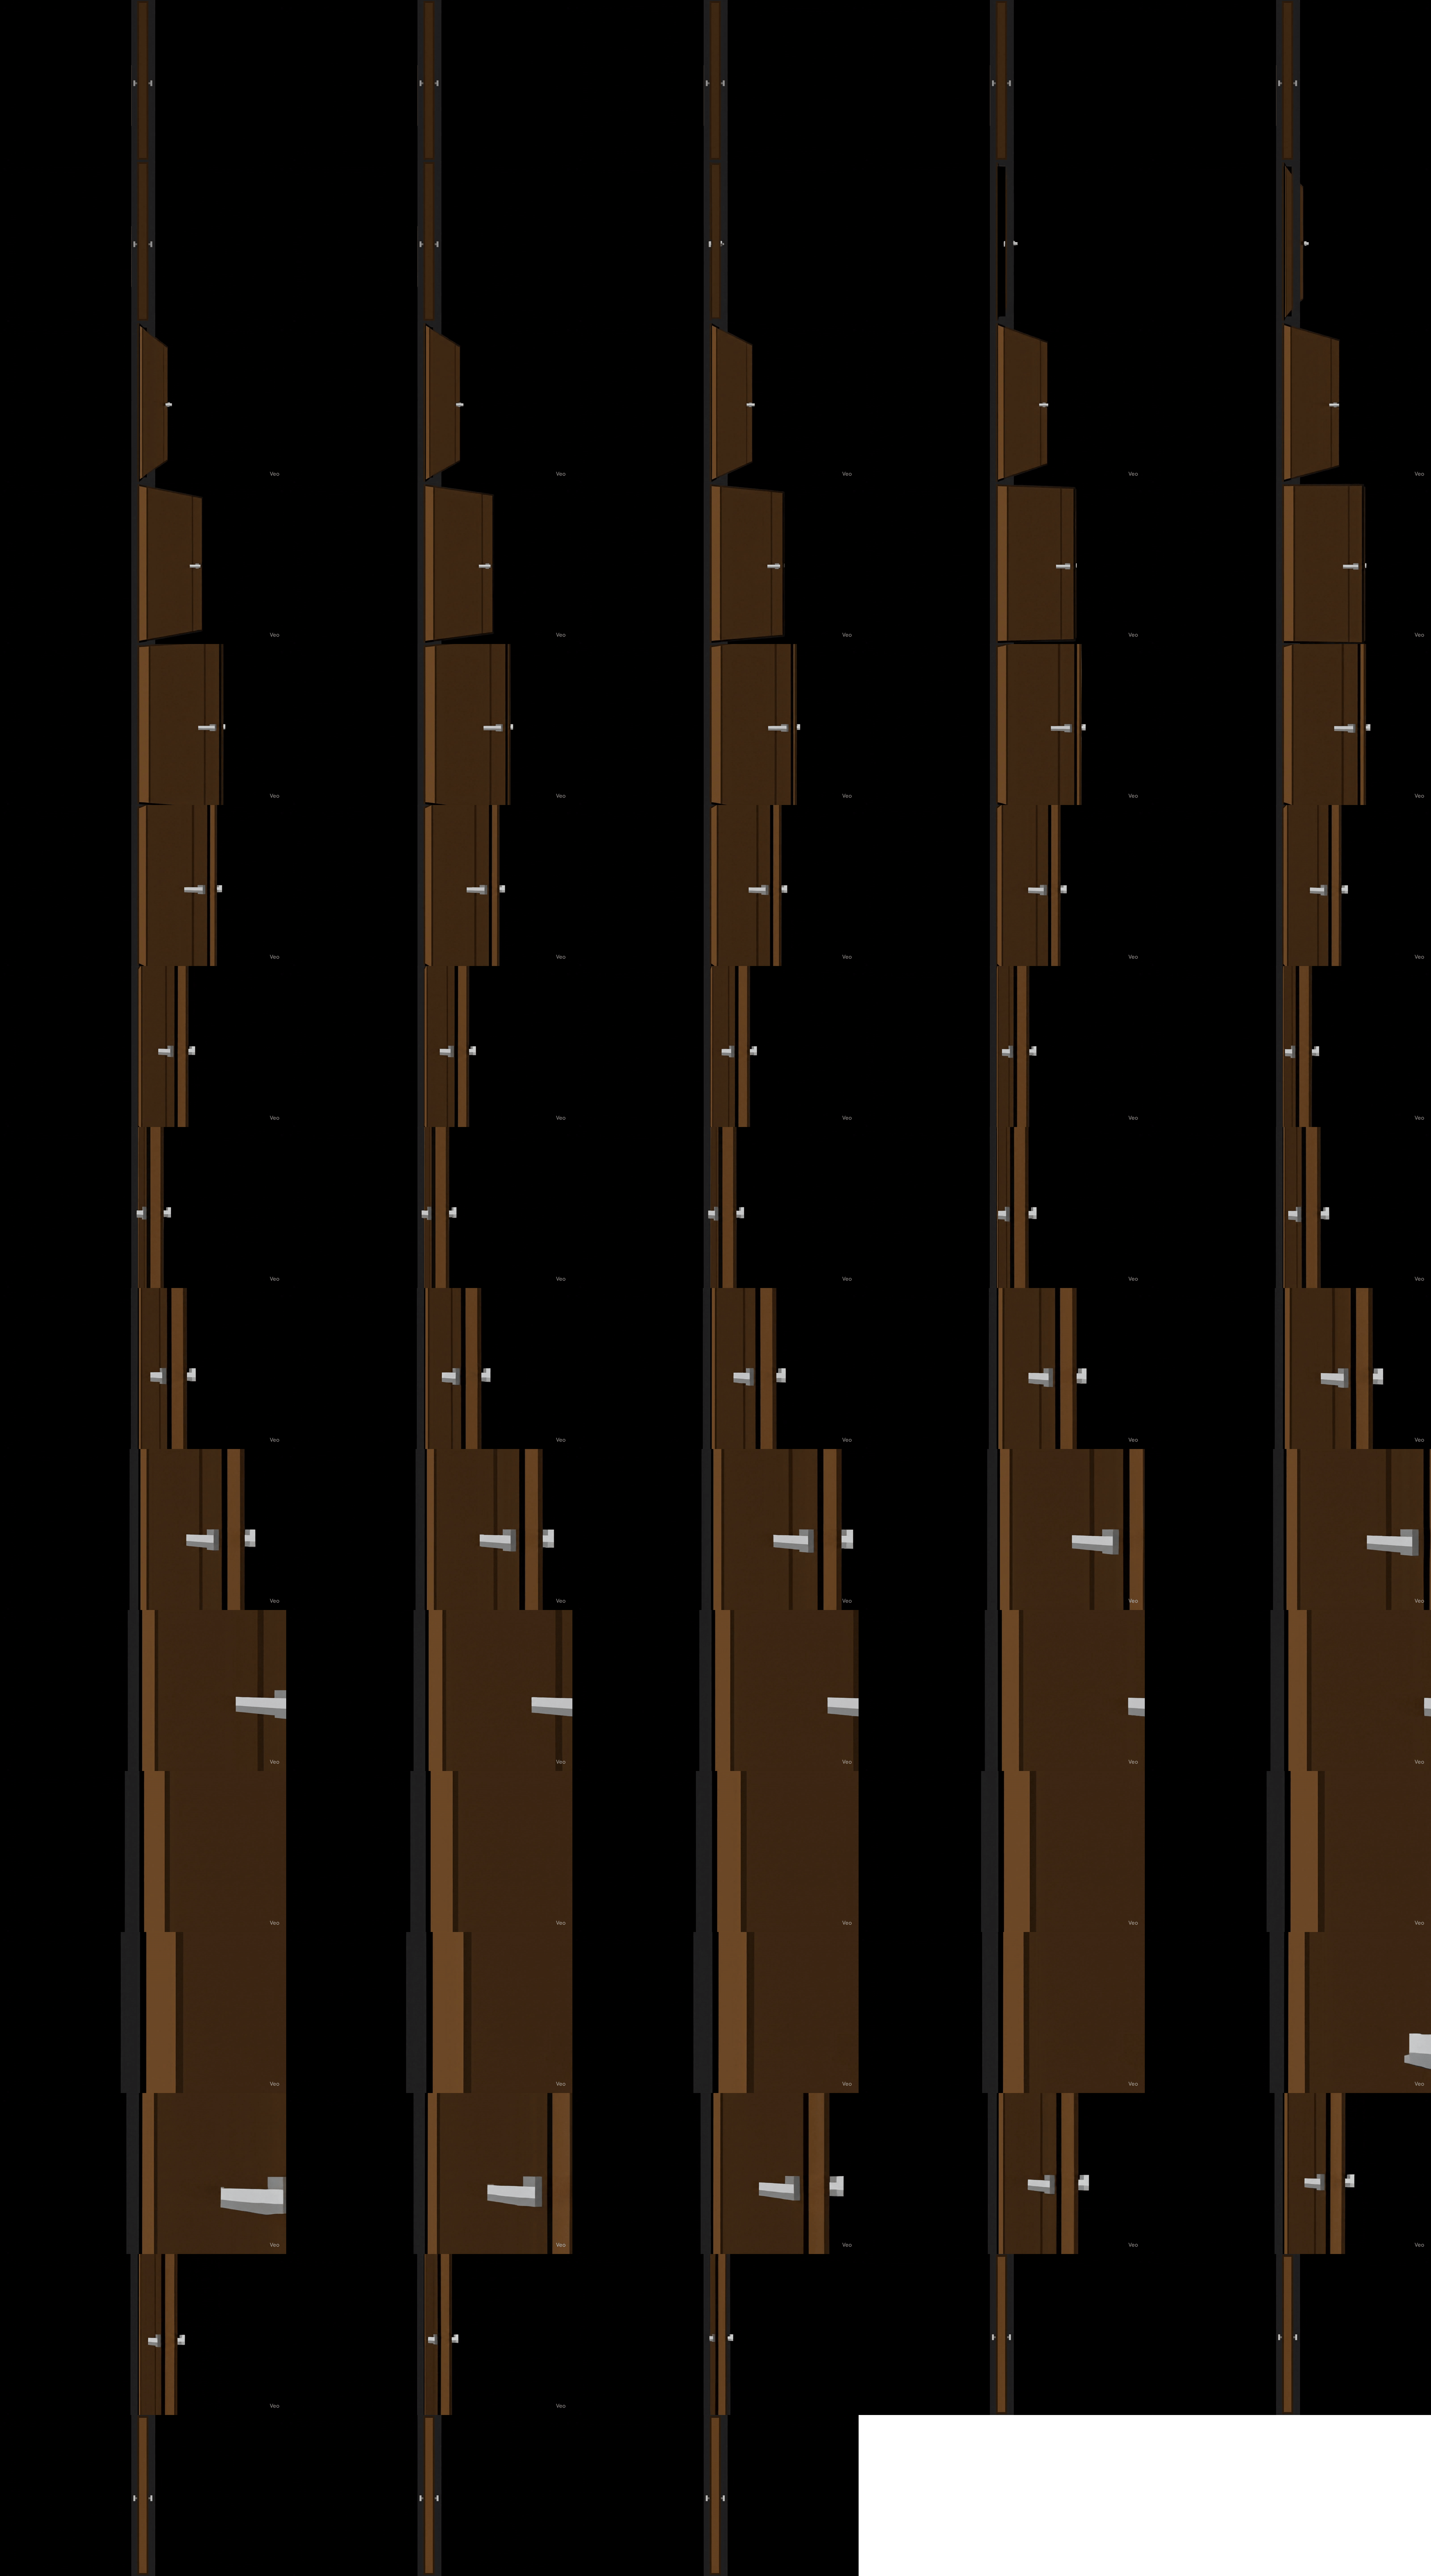
\includegraphics[width=0.7\linewidth]{figs/geminiPro/sprite sheet/side_door_sprite_sheet.png}
    \legend{\small Fonte: Elaborada pela autora, utilizando a ferramenta ezgif.}
\end{figure}

\begin{figure}[htbp]
    \centering
    \caption{\small Sprite sheet sem fundo e pixelizado da animação da Porta B abrindo gerada no Gemini Pro}
    \label{fig:geminiProPortaBSpriteSheetPixel}
    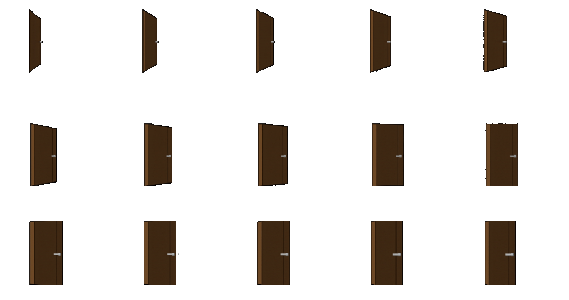
\includegraphics[width=1\linewidth]{figs/geminiPro/sprite sheet/side_door_pixel.png}
    \legend{\small Fonte: Elaborada pela autora, utilizando a ferramenta Pixilart.}
\end{figure}

